
\section{Control model of longitudinal and angular degrees of freedom}
\label{sec:III} 

We will now extend our analysis to additional degrees of freedom. Experimentally, a torsion pendulum suspension is  easy to build. Therefore we will focus our attention to controlling the yaw motion of a test mirror, keeping in mind that the method can be applied to any additional degree of freedom. For actively controlling two degrees of freedom (length and yaw), we need a two-dimensional control system. In other words, we will need a second dual-carrier optical spring in a setup that for example looks like Fig.\ref{fig:angular}. We will label the two dual-carrier optical fields as beams $A$ and $B$. Each beam includes a carrier and a sub-carrier field, i.e.
\begin{eqnarray}
\label{eqn:beams}
\mbox{Beam A = carrier A + sub-carrier A}\\ \nonumber
\mbox{Beam B = carrier B + sub-carrier B}\nonumber
\end{eqnarray}
The two beams have a different optical axis, and each has its own optical spring constant, $K_{OS}^A$ and $K_{OS}^B$, given by equation 
\ref{eqn:KOSsum}.

If we define $x_A$ and $x_B$ as the longitudinal displacement of the mirror at the contact points
of beam A and beam B on the test mirror,
 %the position of the mechanical system at the attachment point of \tcr{incidence of} beam $A$ and beam $B$ \tcr{on the %test mirror}, 
 and $F_A$ and $F_B$ as the corresponding exerted forces, we can describe the mechanical system with a plant matrix $M$:
\begin{equation}
 \begin{pmatrix}
x_A\\ x_B
\end{pmatrix} 
=
M \begin{pmatrix}
F_{A}\\ F_{B}
\end{pmatrix}
\label{eq:MF}
\end{equation}
The explicit expression for $M$ for a torsion pendulum is given in appendix \ref{app:B}.

The control is provided by the optical springs. In the $x_A$-$x_B$ basis the control matrix $H$ is diagonal and given by  (also see Fig.\ref{fig:block_loops})
\begin{equation}
\begin{pmatrix}
F_{A}\\ F_{B}
\end{pmatrix}
= H
 \begin{pmatrix}
x_A\\ x_B
\end{pmatrix} 
=  \begin{pmatrix}
K_{OS}^A & 0 \\ 0 & K_{OS}^B
\end{pmatrix} 
 \begin{pmatrix}
x_A\\ x_B
\end{pmatrix} 
\label{eq:HX}
\end{equation}

\begin{figure}[t]
	\centering
		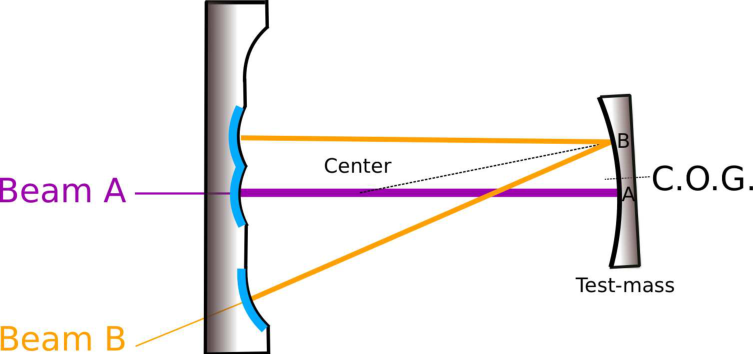
\includegraphics[width=10cm]{./figures/trap_drawing_paper2.pdf}
	\caption[Angular Trap Sketch]{
	In this sketch the main purple (Beam A) optical axis hits the test mirror %only slightly off-center 
	at point A, slightly displaced from the center of gravity (C.O.G.), such
	 that it still corresponds mainly to the length degree of freedom. Thus the second orange (Beam B) optical axis, which hits the test mirror closer to the edge at point B, needs much less power to balance the total DC torque. In our test setup the large input coupler is a composite mirror. It is 600 times more massive than the small mirror. The choice of a V-shaped beam B results in a more practical spot separation on the input coupler. }	


%with orders of magnitude more mass than the small mirror, 
%in order to ensure two different optical axes rigidly coupled.}	
	%can be as a multiple mirror.}%A monolithic, suspended platform is used for all auxiliary mirrors. %Once both one dimensional optical traps are engaged, i.e. their electrical feedback turned off, the DC alignment of the test mirror can still be adjusted by tuning \tcb{the...AOM frequency.}
	
	\label{fig:angular}
\end{figure}



\begin{figure}[htbp]
	\centering
	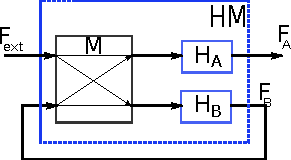
\includegraphics[width=10cm]{./figures/block_mimo_paper.pdf}
	\caption[Multi-Dimensional Mechanical Transfer Function]{
        Block diagram of beam A and beam B. The transfer function $F_A/F_{ext}$ is equal to $OL_A$ from equation \ref{eq:2dol}. Each loop affects the other resulting in cross terms
	present in the matrix $HM$. $M$ and $H_{A,B}$ are the transfer functions of the mechanical system and the optical springs of beam A and B, respectively.}
	\label{fig:block_loops}
\end{figure}

%\tcb{The model includes two optical cavities, referred to as beam A and B, both with an optical finesse of 104. 
%	The main cavity (beam A) is pumped with 0.8 Watt of carrier light, detuned by 36 kHz (blue detuning), and 0.2 
%	Watt of sub-carrier light, detuned by 12 kHz (red detuning). This produces a statically and dynamically stable 
%	optical spring with a lever arm of 1.3 mm, measured from the payload center of gravity. A second optical spring 
%	(beam B) is pumped with 16 times less power, but is otherwise similar to beam A. This side cavity has a lever 
%	arm of 2 cm on the payload, such that the DC radiation pressure torques of beam A and B cancel. The DC radiation 
%	pressure force is canceled by displacing the position pendulum.}

%\subsection{Method}
%\tcb{remove subsection}
For a multi-dimensional feedback system to be stable, it is sufficient that each individual (one-dimensional) feedback loop is stable, assuming all remaining control loops are closed. In other words, in our two-dimensional opto-mechanical system, we close the beam $B$ control filter for evaluating the open loop transfer functions $OL_{A}$, and vice versa. For the open loop transfer functions $OL_{A}$ and $OL_{B}$ we then find: 
\begin{eqnarray}
\label{eq:2dol}
OL_{A}=e_A^{T}\left(\mathds{1}-HM (\mathds{1} - e_A e_A^T) \right)^{-1}HMe_A  \\
OL_{B}=e_B^{T}\left(\mathds{1}-HM (\mathds{1} - e_B e_B^T) \right)^{-1}HMe_B \nonumber
\end{eqnarray}
with $e_A^T=(1,0)$ and $e_B^T=(0,1)$. The derivation of this expression is given in appendix \ref{app:C}.


%%%%%%%%%%%%%%%%%%%%%%%%%%%%%%%%%%%%%


\subsection{An Example}

It is worth considering a specific set of possible values for our model and evaluate the control of  angular and longitudinal degrees of freedom of a gram-scale test mirror using the radiation pressure of the light.
All the optical fields involved in our analysis are derived from the same wavelength light source through frequency shifting.
The model includes two optical cavities (Fig.\ref{fig:angular}), referred to as beam A and B, both with an optical finesse of  about $8000$ and linewidth $\gamma/(2 \pi) = 110\,$kHz. 
The main cavity (beam A) is pumped with $1\,$W of carrier light, detuned by $\delta/(2 \pi)= 250\,$kHz (blue detuning, $\delta/\gamma = 2$), and $0.2\,$W of sub-carrier light, detuned by $\delta/(2 \pi) =60\,$kHz (red detuning, $\delta/\gamma = -0.5$). This produces a statically and dynamically stable optical spring with a lever arm of $0.8\,$mm, measured from the payload center of gravity (C.O.G.). A second optical spring (beam B) is pumped with 6 times less power of carrier light, detuned by $=186\,$kHz (blue detuning, $\delta/\gamma=1.5$), and $40\,$mW of sub-carrier light, detuned by $60\,$kHz (red detuning, $\delta/\gamma=-0.5$). This side cavity has a lever arm of $3.3\,$mm on the payload, such that the DC radiation pressure torques of beam A and B cancel. The DC radiation pressure force can be canceled by displacing the position pendulum.

\begin{figure}[htbp]
	\centering
		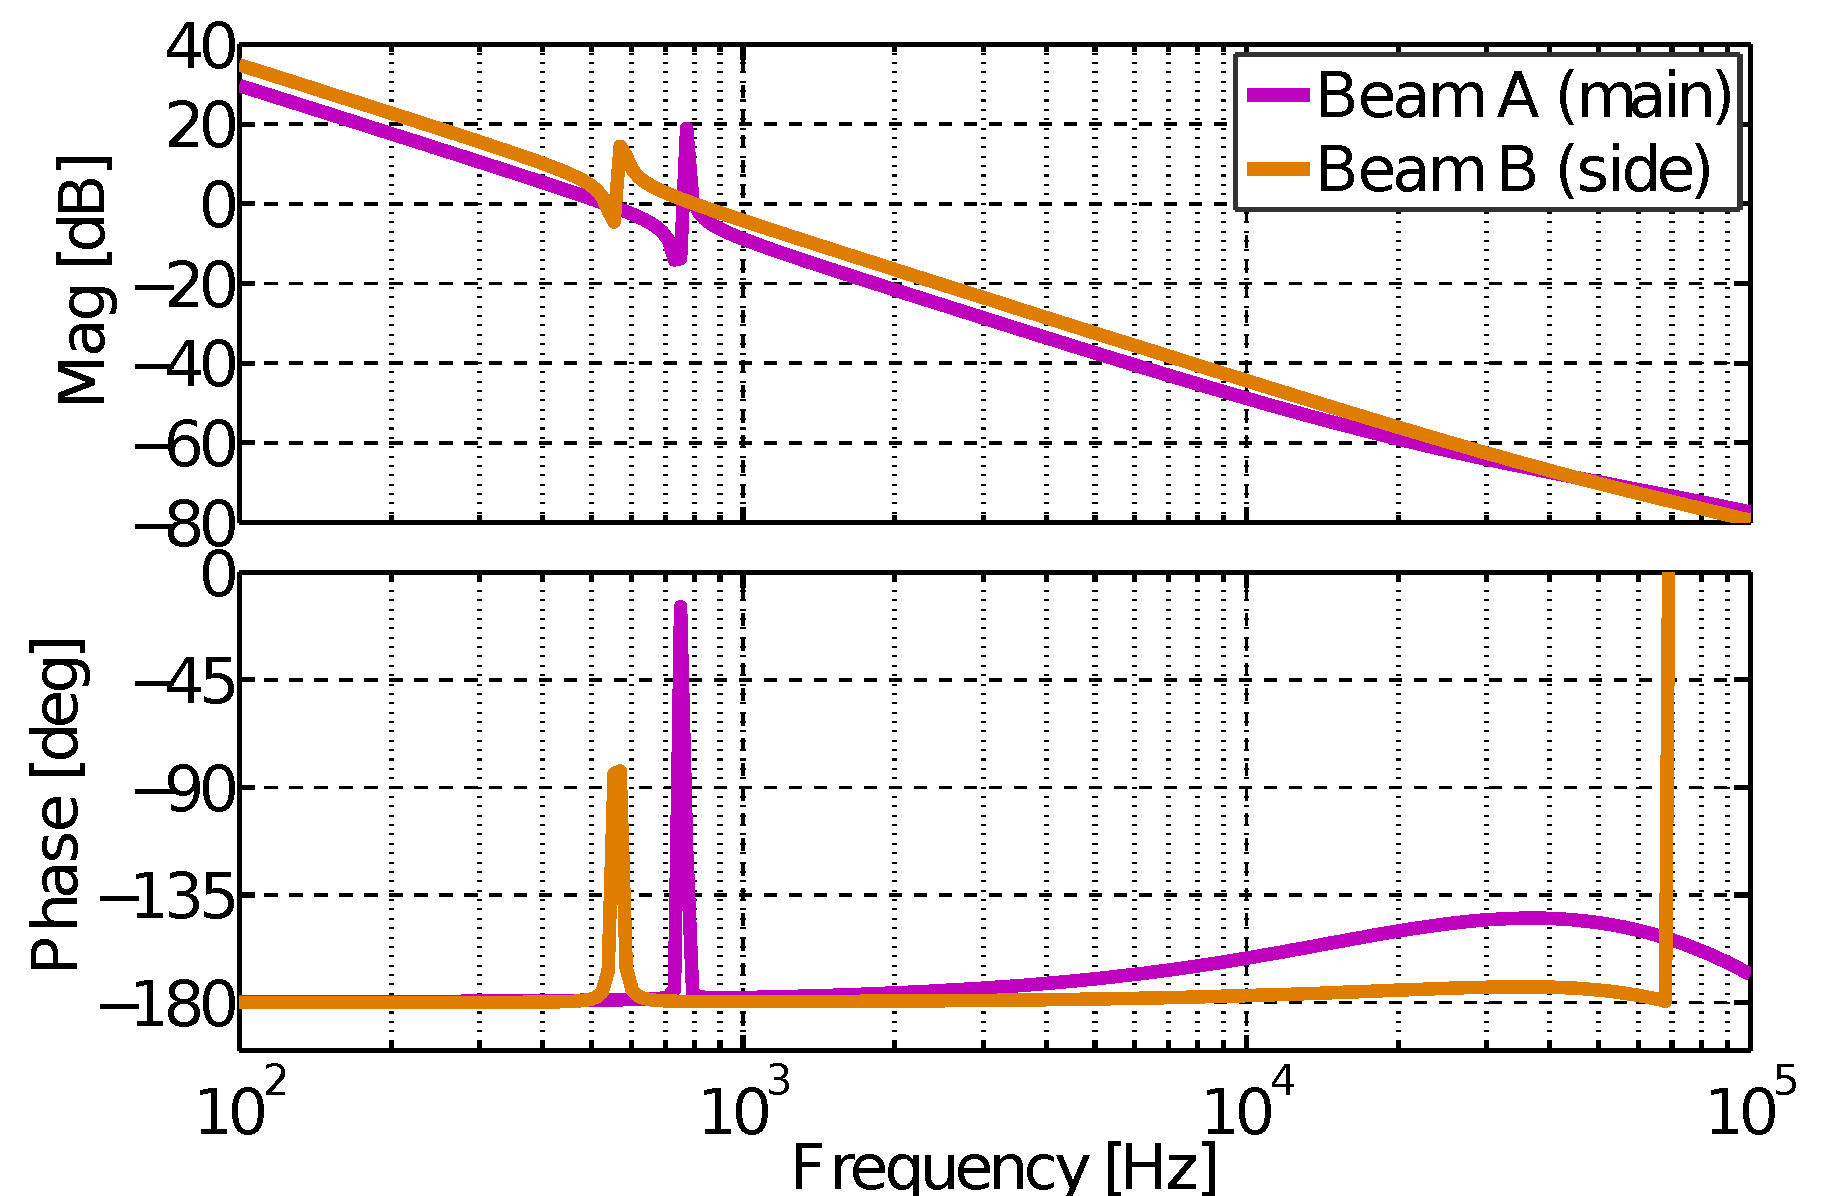
\includegraphics[width=10cm]{./figures/open_loops_TF_paper2.pdf}%filename.pdf}%
		%\includegraphics[width=8cm]{./images/filename.pdf}%
	\caption[Cavity Open Loop Gains]{{
        Open loop gain (OLG) for the main and side cavity.	The respective other loop is closed, and shows up as a resonance in the OLG. Note that, despite multiple unity gain crossings, both loops are stable because the resonances effectively implement a lead filter and the OLG avoids the critical point -1. Thus the dynamic interplay between multiple trapping beams on one payload does not introduce an instability.}}
	\label{fig:control_loops}
\end{figure}


The stability of the combined two-dimensional system is addressed in Fig.\ref{fig:control_loops}. Plotted are the open loop gain functions of the two degrees of freedom (the two optical traps) under the assumption that the other loop is closed. The presence of the second loop introduces a resonance feature in each loop at the unity gain frequency of the other loop. However the open loop gain avoids the critical point -1 (phase at zero), leading to a stable system. The model parameters were intentionally tuned for low damping / high quality factor in order to demonstrate that the system remains stable. Lower quality factors, and therefore stronger cooling is easily achievable.

%If we consider the cavity with both loops closed and we scan one of the mirror we obtain the stability region showed
%in Fig.\ref{fig:stability_region}. The green shaded area represents the offset range of the cavity length at which the two loops remain still stable. The range is $\backsim 20\,$pm.
%
%\begin{figure}[htbp]
%	\centering
%		\includegraphics[width=9cm]{./images/DC_offset}
%	\caption{{(Left) Static carrier and sub-carrier build-up as function of mirror position: Plotted are carrier and sub-carrier build-up (calibrated in Newton of radiation pressure) as a function of the respective cavity position. Also shown in blue is the total force. The trap is both statically and dynamically stable in the green shaded area.
%	%In Figure 4 the static (DC) radiation pressure force due to each of the four laser fields is plotted 
%%as a function of cavity position. Indicated by green shading are the regions with a stable optical 
%%spring (statically and dynamically). 
%With the chosen model parameters those regions are about 
%20 picometers wide.}}
%	\label{fig:stability_region}
%\end{figure}


\subsection{Stability range}
\label{sec:stability}
%\input{OT_paper_stabrange.tex}
We can now estimate the robustness of our feedback control system 
by changing the microscopic length $\delta x_A$ and $\delta x_B$ of the two cavities. This changes the detuning of the optical springs for both beams. Therefore the propagators $X_A$ and $X_B$ for both beams change according to $X_{A,B}=r_1r_2 e^{-i\delta_{A,B}\tau_{A,B}}\cdot e^{ik\delta x_{A,B}}$. For each position both the static and dynamical stability of the total optical spring system given by equation \ref{eq:2dol}
%s \ref{KOS_full_2}, \ref{eqn:K0} and \ref{eqn:KOSsum}
is reevaluated.
%For beam A (and similarly for beam B) we correct the optical spring introducing the additional $\delta x$ to the propagator $X$, becoming $X=r_1r_2 e^{-i\delta\tau}\cdot e^{ik\delta x}$, the optical springs for both beams $i=A,B$ become
%\begin{eqnarray}
%\label{eqn:Koffset}
%K_{OS}^i = K_{OS}^{c_i} + K_{OS}^{sc_i} \approx -2 \eta r_1r_2 \tau(\delta_c+\delta_{sc})k\delta x 
%K_{OS}^B = K_{OS}^{cB} + K_{OS}^{scB} \approx -2 \eta r_1r_2 \tau(\delta_c+\delta_{sc})k\delta x
%\end{eqnarray}
%and we check the stability with the same procedure described in Section(bla) at different values of the offset. 
%at each single value of the cavity lengths. 

In Fig. \ref{fig:stability_region} the radiation pressure force due to the intra-cavity power of both beams
versus the cavity offset is shown. The green shaded area represents the position range in which the two loops remain stable.  The range is $\backsim 20\,$pm. 
The DC force fluctuations that the system can tolerate are given by the y-axis interval that the blue curve spends in the green shaded area. %{\color{red} The range is about $xx N$ for beam A and about $yy N$ for beam B. }

\begin{figure}[htbp]
	\centering
		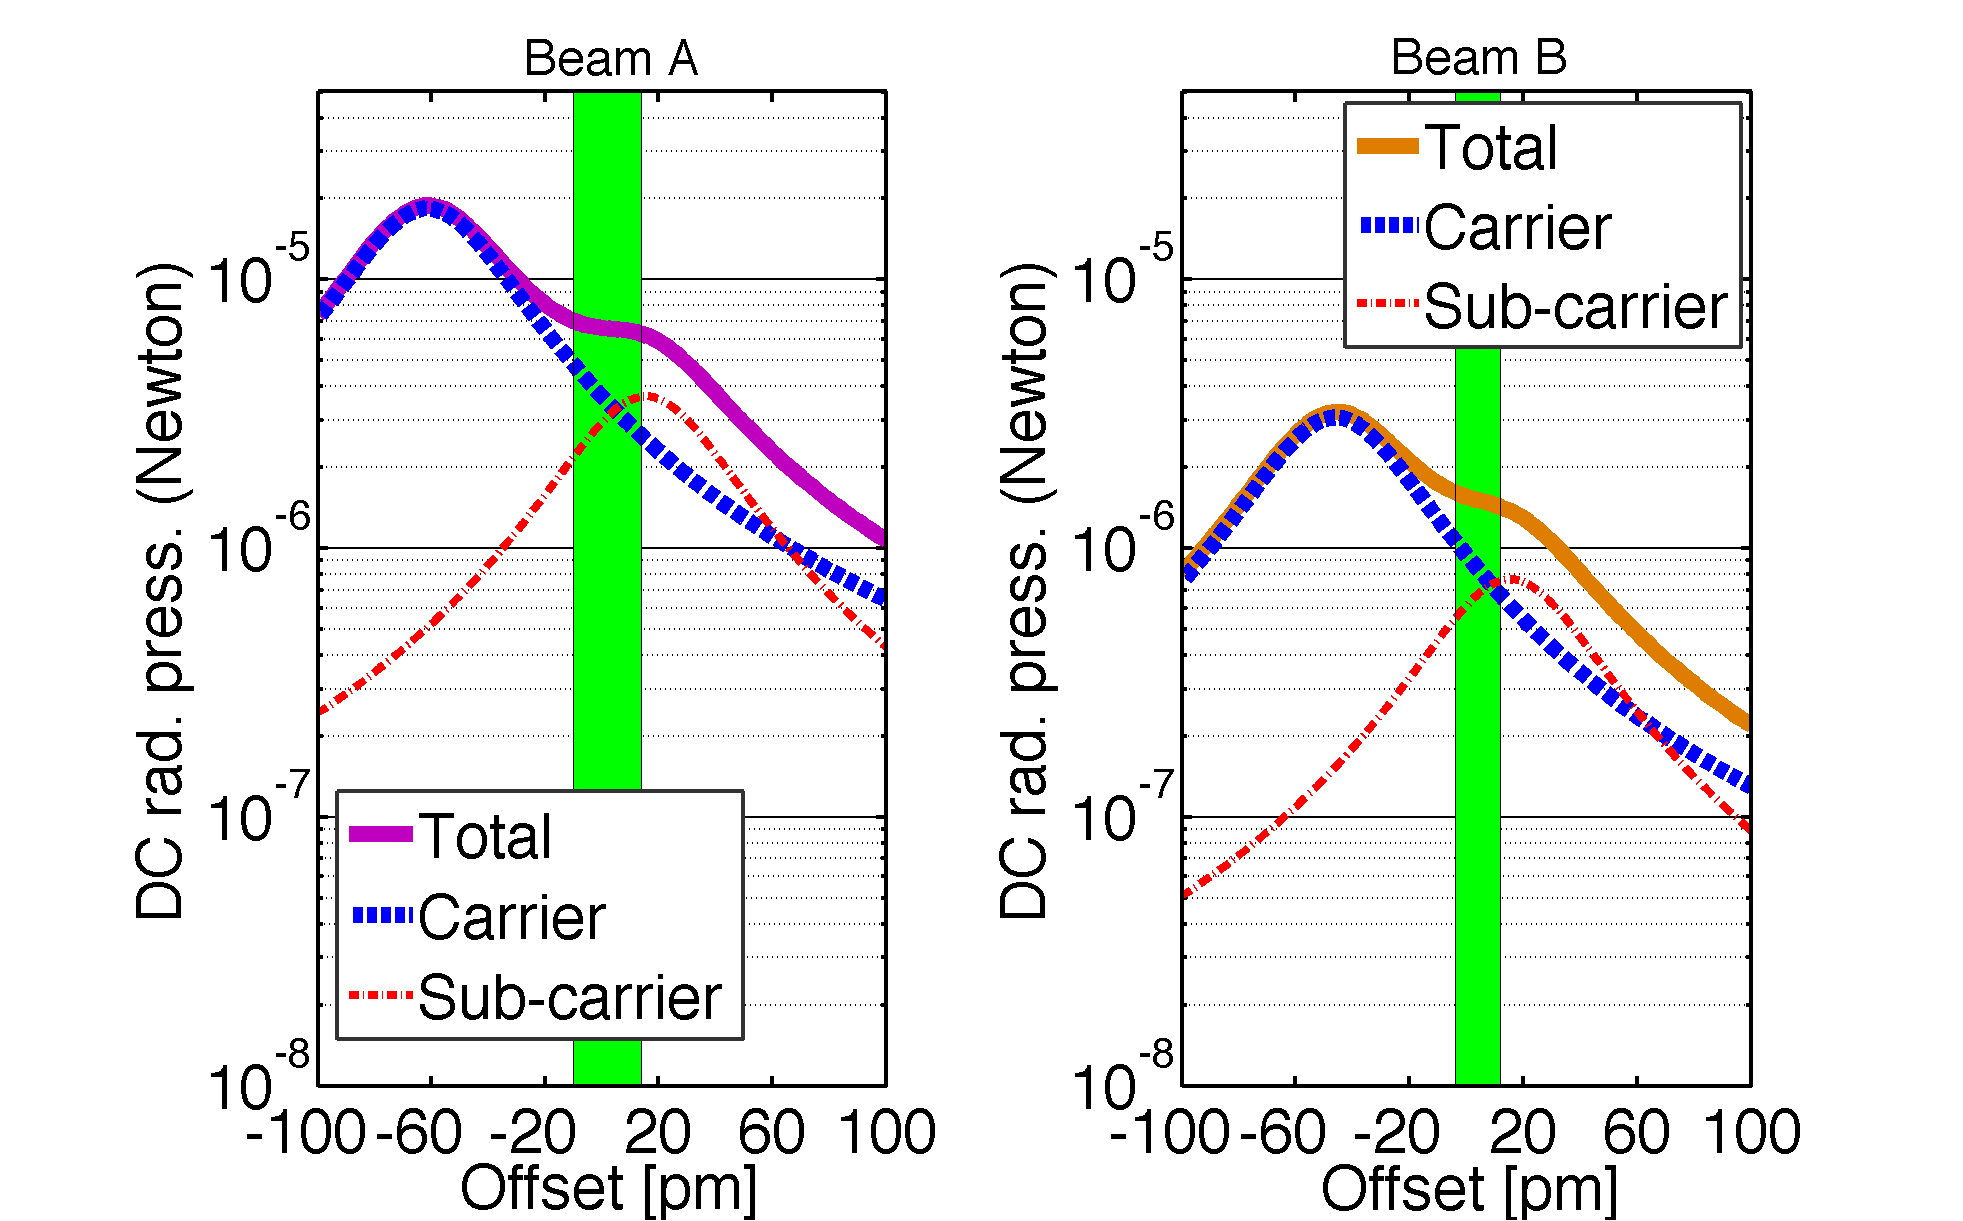
\includegraphics[width=10cm]{./figures/DC_offset_paper3.pdf}
	\caption[Stability Range]{{
        Static carrier and sub-carrier build-up (calibrated in radiation pressure force) as a function of the respective cavity position. Also shown in blue is the total radiation pressure force. Using the stability testing method from section \ref{sec:stability} we find that the trap is both statically and dynamically stable in the green shaded area.
	%In Figure 4 the static (DC) radiation pressure force due to each of the four laser fields is plotted 
%as a function of cavity position. Indicated by green shading are the regions with a stable optical 
%spring (statically and dynamically). 
With the chosen model parameters those regions are about 
20 picometers wide.}}
	\label{fig:stability_region}
\end{figure}

%\tcb{Finally, Fig...... shows a simple noise budget for this MATLAB model. It is calibrated in actual motion after the trap closed loop gain suppression. The seismic noise estimate is based on a typical ground motion filtered by a one-stage passive isolation platform with a resonance frequency of $1\,$Hz. It results in a residual RMS motion of about 1 picometer. This is smaller than the 12 picometer stability band shown in Figure 4. Therefore it should be possible to turn off any feedback to the cavity length or laser frequency. The two cavities will remain locked purely due to the radiation pressure trapping force, thus trapping the payload.}


